\subsection{Stacks and queues}

Stacks and queues are the containers we will use here.
They are very similar in nature, and they are both special cases of
\emph{deques}, double-ended queues, but they will make a huge difference
in the order of exploration.

Deques are lists that allow insertion, access and deletion
of elements on both ends, in constant time.
We will not worry about the implementation here.

A \emph{stack} only allows insertion, acess and deletion
at the back of the list.
We can view it as a stack of pancakes: you can only add or remove a pancake
at the top of the pile.
It follows the \emph{LIFO} (last-in-first-out) principle:
the last element that is inserted is the first to be processed.
\begin{center}
    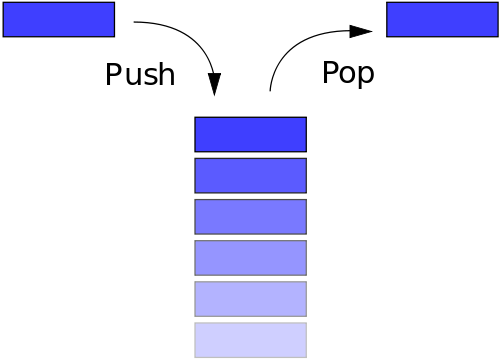
\includegraphics[width=0.3\textwidth]{img/stack}
\end{center}

A \emph{queue}, on the other hand allows insertion only at the back,
while acess and deletion only happen at the front.
We can view it as a queue at the checkout in a store.
It follows the \emph{FIFO} (first-in-first-out) principle:
the elements are processed in the same order that they were inserted.
\begin{center}
    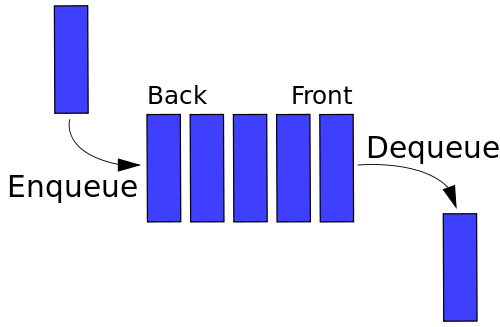
\includegraphics[width=0.3\textwidth]{img/queue}
\end{center}

The corresponding function members are \texttt{.push()} for insertion,
\texttt{.pop()} for deletion and for acess, stacks have \texttt{.top()}
and queues have \texttt{.front()}.
